\chapter{Sequence Context Effect}\label{sce}

Different cancers develop under the influence of different conditions, especially mutagens and repair systems, thus each cancer type possesses a distinctive mutation composition. Base substitutions have been shown to exhibit an association with distinct patterns of neighbouring bases \citep{Zhu2017,Zhu2020,Vinson2012CGMethylation}. This is the premise of most commonly employed methods for cancer classification. The question is whether flanking bases beyond 3-mers, specifically positions -2 \& +2, have an influence on whether the mutations occur. Using the statistical measure of in formation \gls{re}, this chapter evaluates the importance of both the composition of base substitutions and their flanking bases in characterising mutagenesis in cancer. Above all, the chapter shows that the \gls{sce} was not just contributed by immediate flanking bases (\textit{i.e.} 3-mers). Rather, there was certain value in factoring larger sequence contexts into analysing cancer mutation composition.

\section{Base substitutions were indicative of cancers}
SCE consists of two components, the middle base substitutions and the flanking bases. This section focuses on the first component.

\subsection{Base substitutions were a rich source of information}
To explore the patterns of base substitutions and their potential contribution to SCE, I measured the information available in all base substitution types for all cancers using relative entropy $RE$'s. Specifically, $RE$'s were computed using a pair of generalised linear models (GLM), a null and a saturated GLM. The null GLM assumed that all substitutions involved occurred at the same rates and the saturated GLM assumed every substitution had a distinctive mutation rate. $RE$'s are a measure of information because they are essentially the information available in the saturated GLM that the null model cannot capture (details in Methods \ref{methods:re} and \ref{methods:spectra}). Four pairs of GLMs were required for the four wildtype bases; therefore, each pair of GLMs output three $RE$'s corresponding to three base substitutions. I plotted $RE$ as ``mutation logos'' in Figures \ref{fig:spectra} and \ref{fig:apdx_spectra}, where the height of the letter is the $RE$ of a base substitution and its orientation dictates whether the substitution is in excess (up) or deficit (down) relative to the null hypothesis. Note that for each cancer (or panel) of Figures \ref{fig:spectra} and \ref{fig:apdx_spectra}, there are four rows, each corresponding to a pair of GLMs for a wildtype base. 

Three features stand out from the plots. First, base substitutions appeared strand symmetric for all examined cancers. That is, $RE$'s were similar for reverse complementary mutations (\textit{e.g.} C$\rightarrow$T and G$\rightarrow$A). Second, the heights of the up-oriented letters for \glspl{transition} (mutations between bases of the same chemical classes) signifies that they were more informative than \glspl{transversion} (mutations between bases of different chemical classes). Third, by visualisation, the patterns of base substitutions were very diverse. For example, Skin-Melanoma was dominated by C$\rightarrow$T/G$\rightarrow$A, but this was not necessarily true in the other cancers (Figure \ref{fig:spectra_skin}). Indeed, Liver-HCC was more strongly characterised by the A$\rightarrow$G/T$\rightarrow$C transitions (Figure \ref{fig:spectra_liver}). For Panc-AdenoCA, the importance of C$\rightarrow$T/G$\rightarrow$A and A$\rightarrow$G/T$\rightarrow$C was roughly the same (Figure \ref{fig:spectra_panc_adenoca}).

\begin{figure}[ht!]
    \begin{subfigure}{.5\textwidth}
    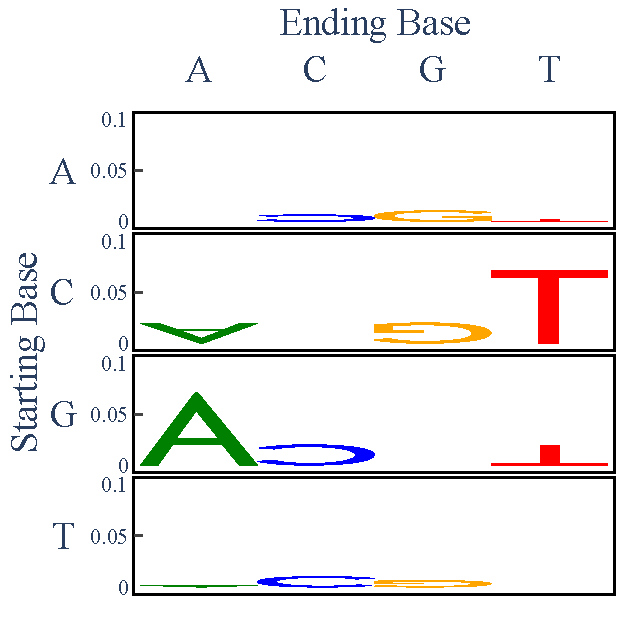
\includegraphics[scale=0.7]{graphics/spectra_Skin-Melanoma.pdf}
    \caption{Skin-Melanoma}
    \label{fig:spectra_skin}
    \end{subfigure}
    ~
    \begin{subfigure}{.5\textwidth}
    
    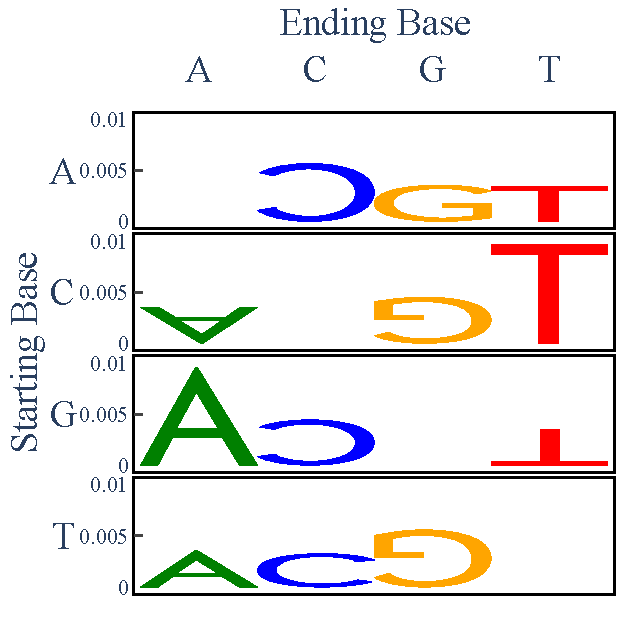
\includegraphics[scale=0.7]{graphics/spectra_Kidney-RCC.pdf}
    \caption{Kidney-RCC}
    \label{fig:spectra_kidney}
    \end{subfigure} \\
    \vspace{0.5cm}
    
    \begin{subfigure}{.5\textwidth}
    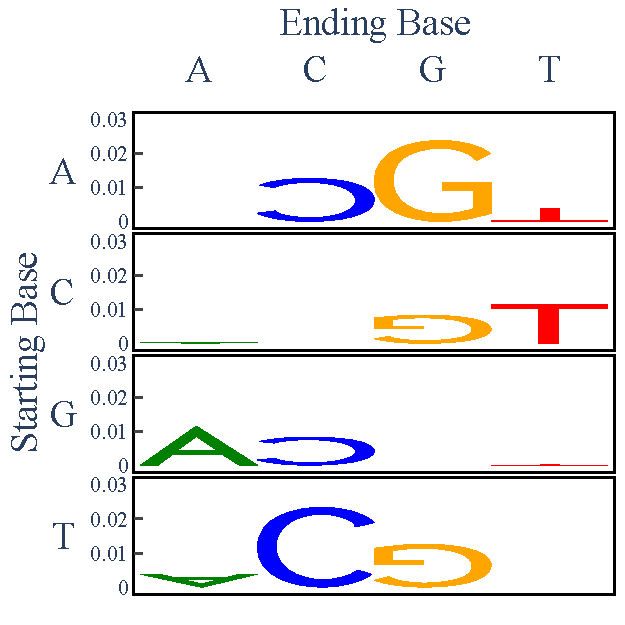
\includegraphics[scale=0.7]{graphics/spectra_Liver-HCC.pdf}
    \caption{Liver-HCC}
    \label{fig:spectra_liver}
    \end{subfigure}
    ~
    \begin{subfigure}{.5\textwidth}
    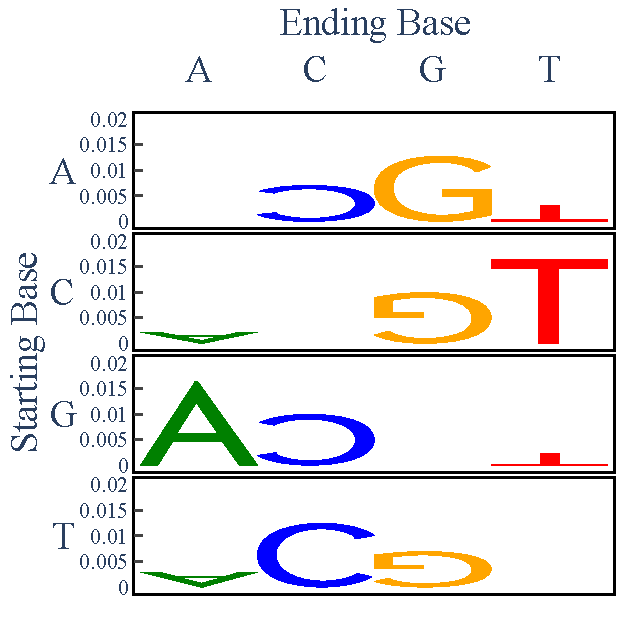
\includegraphics[scale=0.7]{graphics/spectra_Panc-AdenoCA.pdf}
    \caption{Panc-AdenoCA}
    \label{fig:spectra_panc_adenoca}
    \end{subfigure} \\
    \vspace{0.2cm}
    \caption{\textbf{Base substitutions are a rich source of information}. Here, $RE$'s as a measure of information are shown in mutation logos for (a) Skin-Melanoma (b) Kidney-RCC (c) Liver-HCC (d) Panc-AdenoCA. The other cancers can be found in Figure \ref{fig:apdx_spectra}. For each panel, each row was derived from a pair of GLMs corresponding to a wildtype base. The x-axis is the wildtype base; the y-axis is the product of the substitution. The heights of the letters are $RE$'s. An up-orientation indicates an excess while a down-orientation indicates a deficit of the mutation.}
    \label{fig:spectra}
\end{figure}

\subsection{Base substitutions differed between cancers}
To further confirm that base substitutions could distinguish cancers, I performed a hypothesis test for difference between each cancer pair. Similar to the analysis of base substitutions for individual cancers, one such hypothesis test was an aggregation of four pairs of GLMs, each corresponding to a wildtype base. Within each GLM pair, the null GLM assumed their was no difference in the composition of substitutions between two cancers and the alternate GLM assumed the reverse. The four p-values from GLM were combined by Fisher's method to obtain a single joint p-value. The p-values for all pairwise comparisons were adjusted using Bonferroni correction. The detailed methods can be found in Methods \ref{methods:re} and \ref{methods:spectra}.

Most pairwise comparisons were statistically significant, with an exception of CNS-Medullo \textit{v.s.} CNS-PiloAstro, which gave a p-value of 0.63 after Bonferroni correction. The second highest correct p-value was when comparing Lymph-BNHL to Lymph-CLL, at 4.8$\times10^{-20}$. All other p-values were less than $10^{-31}$ Figure \ref{fig:paired_spectra} demonstrates how individual substitutions could contribute to the whole information content of the test. It is no surprise that in Figure \ref{fig:spectra_kidney_skin}, there was a deficit in C$\rightarrow$T/G$\rightarrow$A in Kidney-RCC with respect to Skin-Melanoma, as we have seen previously that the abundance of C$\rightarrow$T/G$\rightarrow$A was somewhat one ``signature'' of Skin-Melanoma. The same can be said about A$\rightarrow$G/T$\rightarrow$C when comparing Kidney-RCC to Liver-HCC (Figure \ref{fig:spectra_kidney_liver}). Additionally, it also is worth noting that the scale of $RE$'s were typically 0.001 to 0.01. In the case of CNS-Medullo \textit{v.s.} CNS-PiloAstro whose p-value was not significant (Figure \ref{fig:spectra_medullo_piloastro}), the $RE$ terms were merely at micro scale ($\mu, 10^{-6}$). This was also true when comparing Lymph-BNHL to Lymph-CLL (Figure \ref{fig:spectra_bnhl_cll}). When comparing any components of the first pairs to the second pairs, $RE$'s were ``restored'' to the normal range (Figures \ref{fig:spectra_piloastro_bnhl} and \ref{fig:apdx_paired_spectra}).

\begin{figure}[ht!]
    \begin{subfigure}{.5\textwidth}
    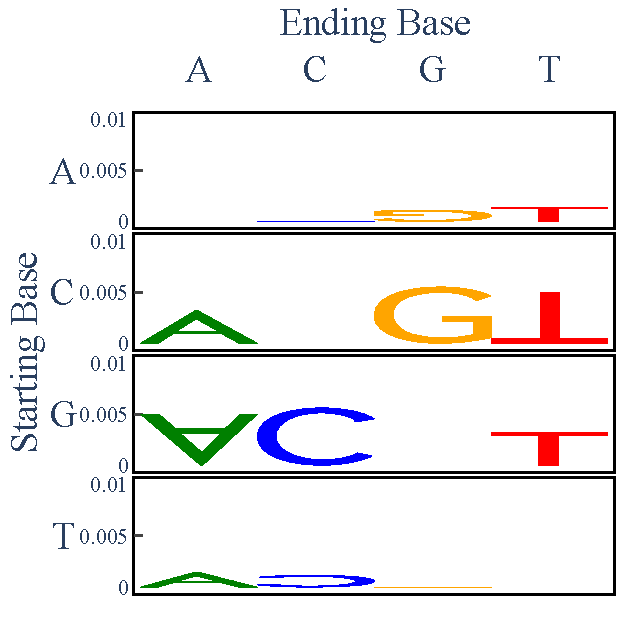
\includegraphics[scale=0.7]{graphics/spectra_Kidney-RCC_Skin-Melanoma.pdf}
    \caption{Kidney-RCC \textit{v.s.} Skin-Melanoma}
    \label{fig:spectra_kidney_skin}
    \end{subfigure}
    ~
    \begin{subfigure}{.5\textwidth}
    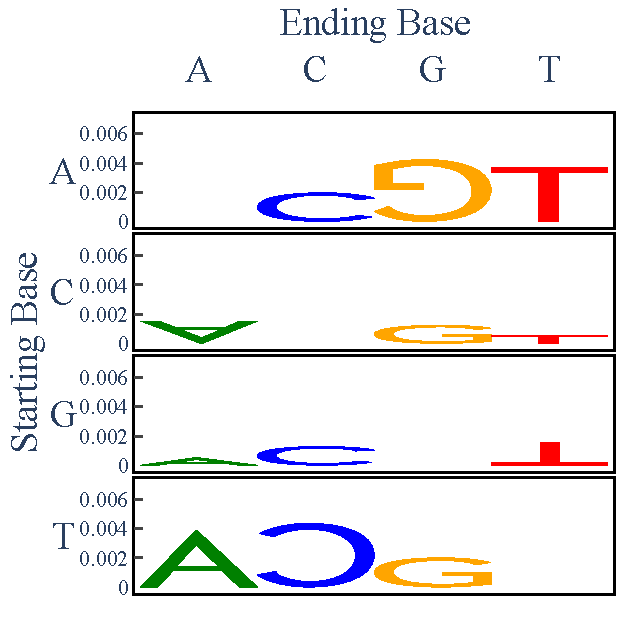
\includegraphics[scale=0.7]{graphics/spectra_Kidney-RCC_Liver-HCC.pdf}
    \caption{Kidney-RCC \textit{v.s.} Liver-HCC}
    \label{fig:spectra_kidney_liver}
    \end{subfigure} \\
    \vspace{0.5cm}
    
    \begin{subfigure}{.5\textwidth}
    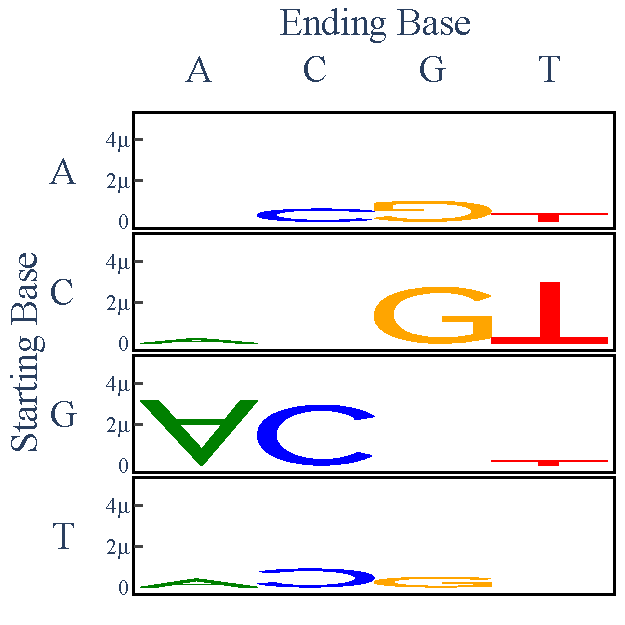
\includegraphics[scale=0.7]{graphics/spectra_CNS-Medullo_CNS-PiloAstro.pdf}
    \caption{CNS-Medullo \textit{v.s.} CNS-PiloAstro}
    \label{fig:spectra_medullo_piloastro}
    \end{subfigure}
    ~
    \begin{subfigure}{.5\textwidth}
    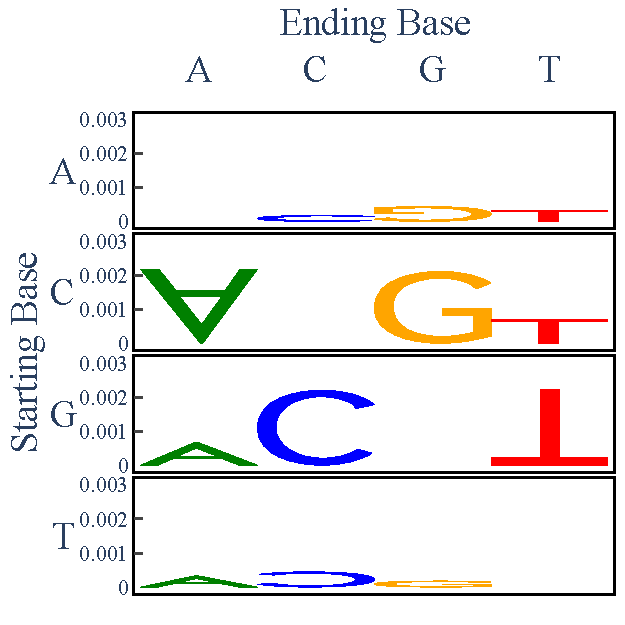
\includegraphics[scale=0.7]{graphics/spectra_CNS-PiloAstro_Lymph-BNHL.pdf}
    \caption{CNS-PiloAstro \textit{v.s.} Lymph-BNHL}
    \label{fig:spectra_piloastro_bnhl}
    \end{subfigure} \\
    \vspace{0.5cm}
\caption{}
    % \caption{\textbf{Base substitutions are promising in discriminating cancers according to $RE$ between cancer pairs.} Similar to Figure \ref{fig:spectra}, for each panel, each row contains the measure of information $RE$ derived from a pair of GLMs. The x-axis is the wildtype base; the y-axis is the product of the substitution. The heights of the letters are $RE$'s. An up-orientation indicates an excess while a down-orientation indicates a deficit of the mutation when comparing the (a) Kidney-RCC to Skin-Melanoma, (b) Kidney-RCC to Liver-HCC, (c) CNS-Medullo to CNS-PiloAstro, (d) CNS-PiloAstro to Lymph-BNHL. More comparisons can be found in Figure \ref{fig:apdx_paired_spectra}.}
    \label{fig:paired_spectra}
\end{figure}

\section{Flanking bases also contained information}
Similar to base substitutions, $RE$ was used to measure the information content in the second component of SCE: the flanking bases. Here, the pair of GLMs recruited to compute $RE$'s included (1) a null GLM assuming the identity of the positions flanking the substitutions was similar to the positions flanking any random bases, provided the wildtype was the same and (2) a saturated GLM assuming they were different. For each cancer, there were 12 pairs of GLMs corresponding to 12 substitutions (details in Methods \ref{methods:re} and \ref{methods:nbr}). As seen previously, transitions were usually more abundant than transversions (Figure \ref{fig:spectra}). For this reason, I plotted $RE$ of the flanking bases for transitions and transversions separately. 

Figure \ref{fig:nbr} shows the results for Skin-Melanoma and Liver-HCC, the rest can be found in Figure \ref{}. As expected, bases flanking transitions contributed more information than bases flanking transversions. Additionally, strand symmetry was also present in the flanking bases. To illustrate, $RE$ for C$\rightarrow$T on position -1 was often approximately of the same level as G$\rightarrow$A on position +1, suggesting a close link between mutations on reverse complementary strands. A very slight deviation from strand symmetry was visible in the transversions of Liver-HCC (Figure \ref{fig:transversion_liver}). Moreover, inner positions (-1 \& +1) contained more information than outer positions, but this does not deny the potentially useful information in the outer positions. In fact, the information from outer positions for transitions were roughly equal to that from inner positions for transversions. Last but not least, the information content was structured differently between Skin-Melanoma and Liver-HCC. For instance, the most informative flanking position for C$\rightarrow$T was position -1 in Skin-Melanoma but +1 in Liver-HCC.

\begin{figure}[ht!]
    \begin{subfigure}{.5\textwidth}
    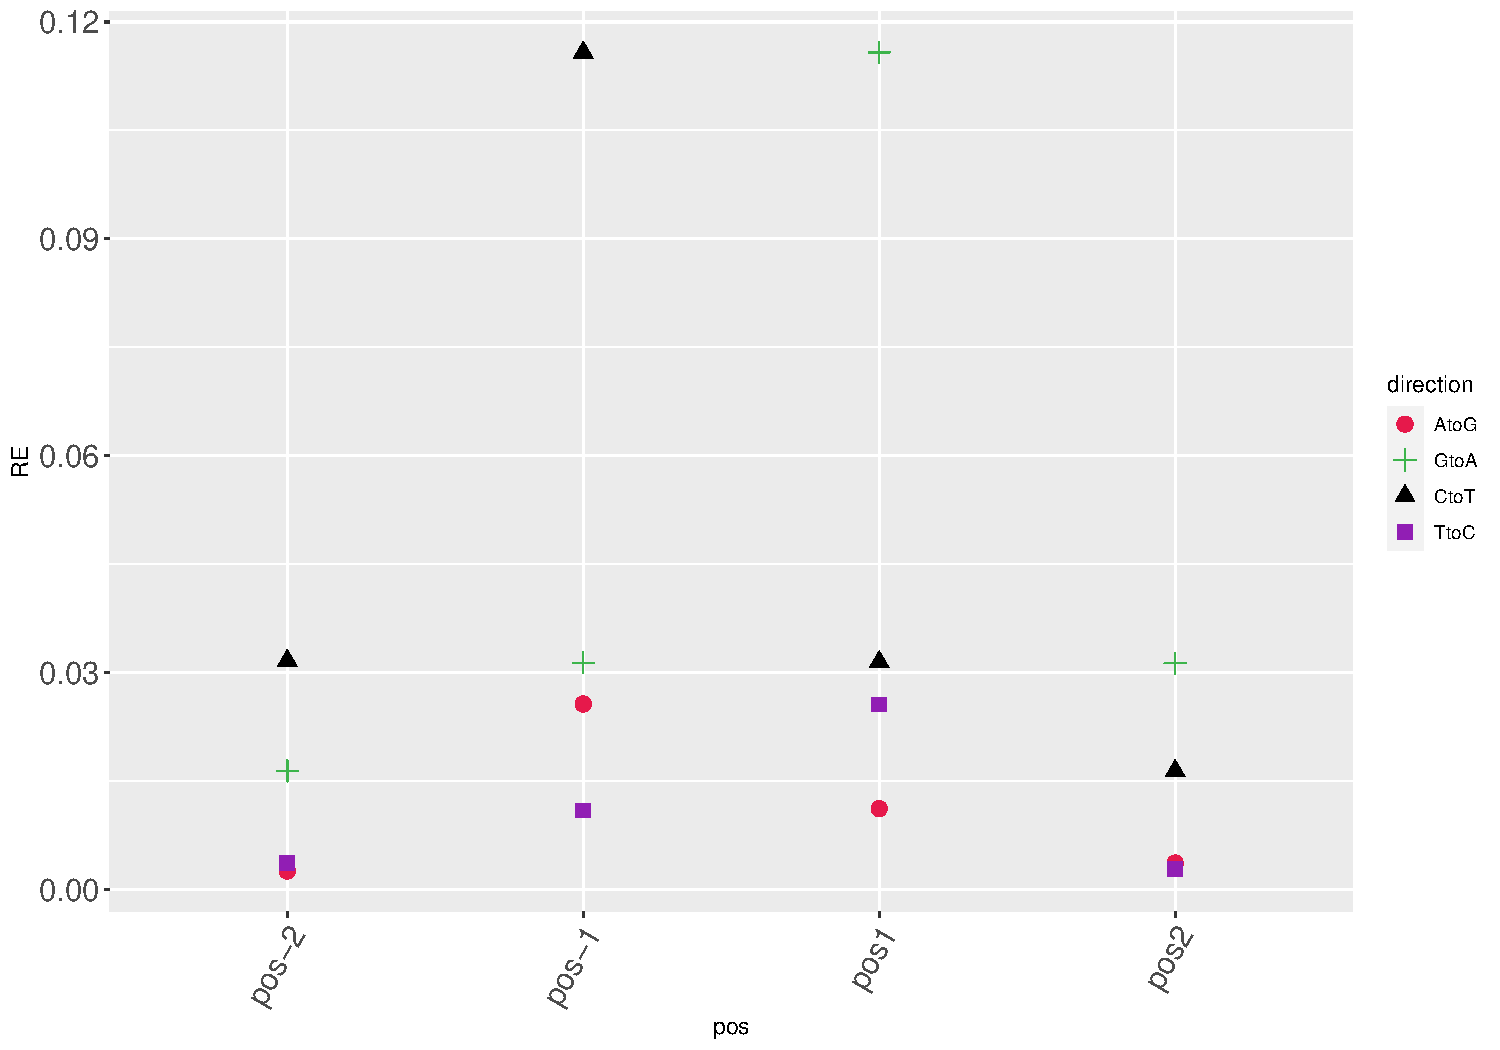
\includegraphics[scale=0.63]{graphics/nbr_transitions_Skin-Melanoma.pdf}
    \caption{transitions/Skin-Melanoma}
    \label{fig:transitions_skin}
    \end{subfigure}
    ~
    \begin{subfigure}{.5\textwidth}
    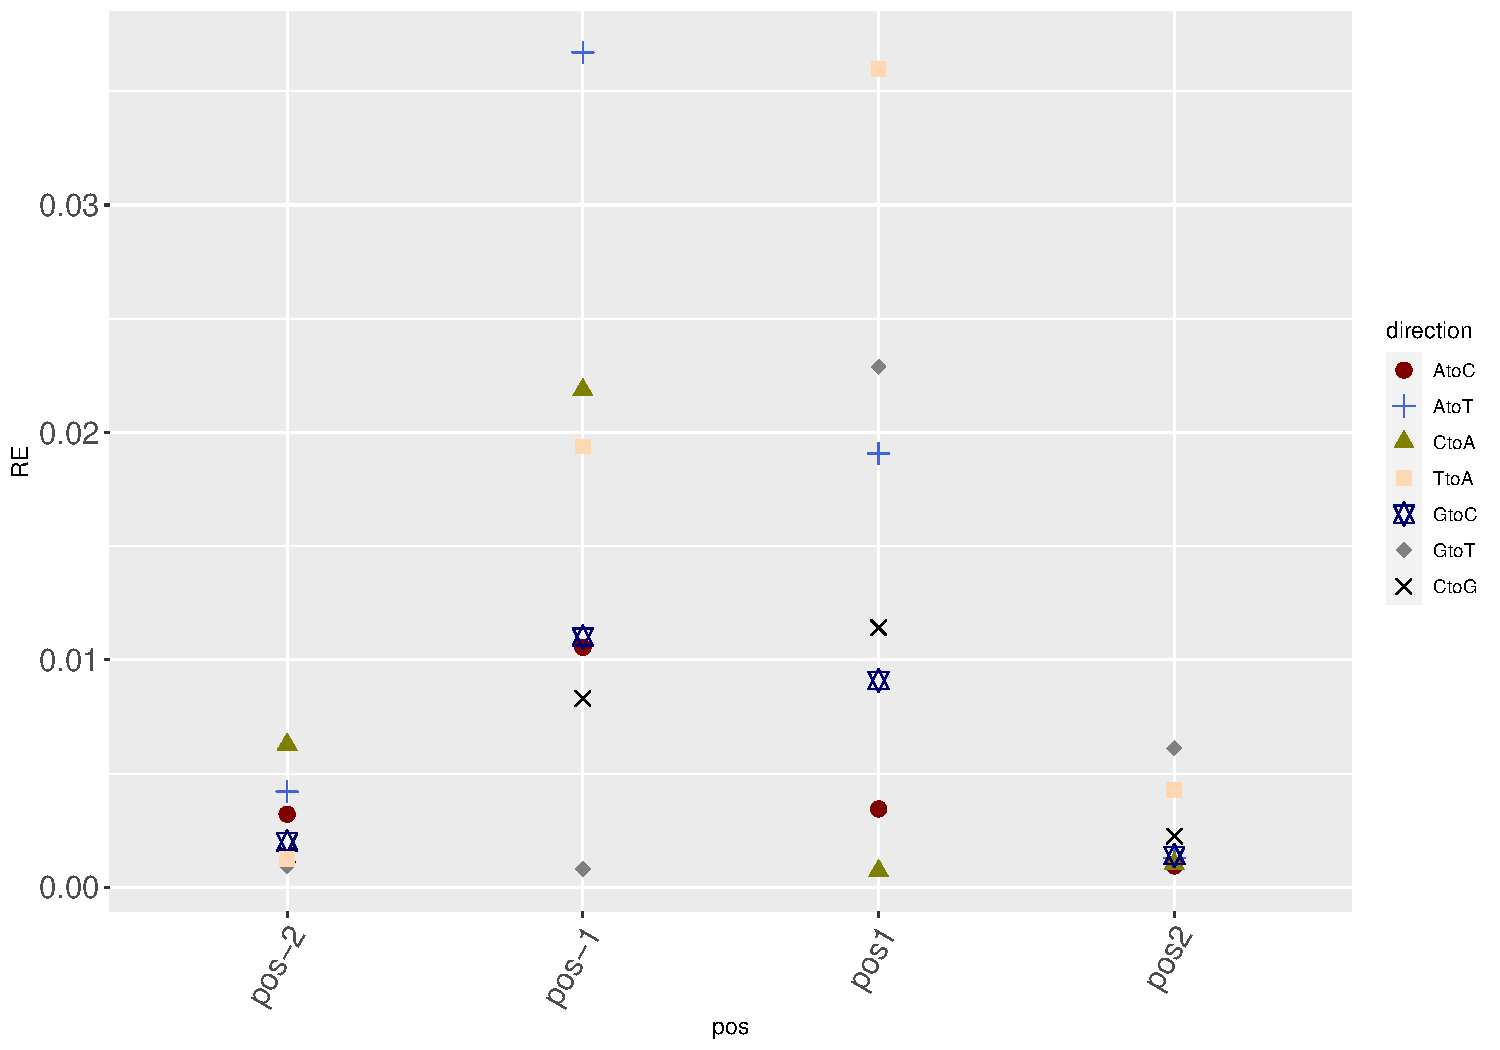
\includegraphics[scale=0.63]{graphics/nbr_transversion_Skin-Melanoma.pdf}
    \caption{transversions/Skin-Melanoma}
    \label{fig:transversions_skin}
    \end{subfigure} \\
    \vspace{0.5cm}
    
    \begin{subfigure}{.5\textwidth}
    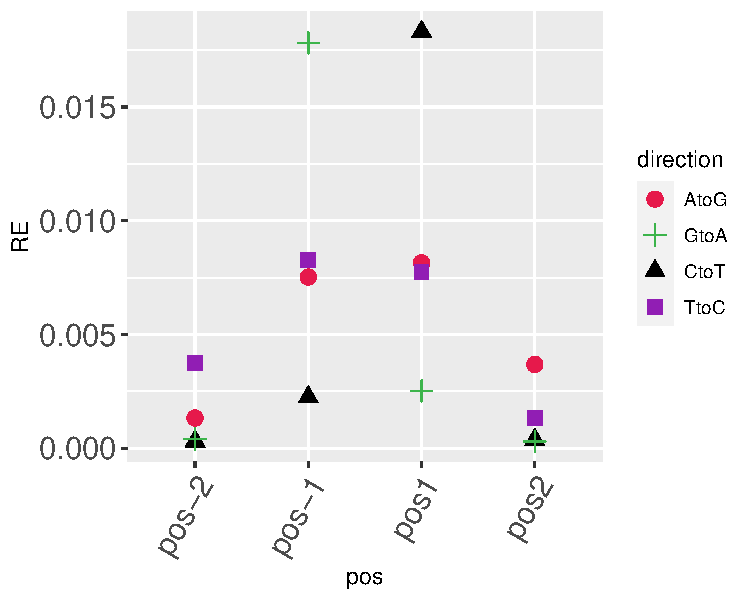
\includegraphics[scale=0.63]{graphics/nbr_transitions_Liver-HCC.pdf}
    \caption{transitions/Liver-HCC}
    \label{fig:transitions_liver}
    \end{subfigure}
    ~
    \begin{subfigure}{.5\textwidth}
    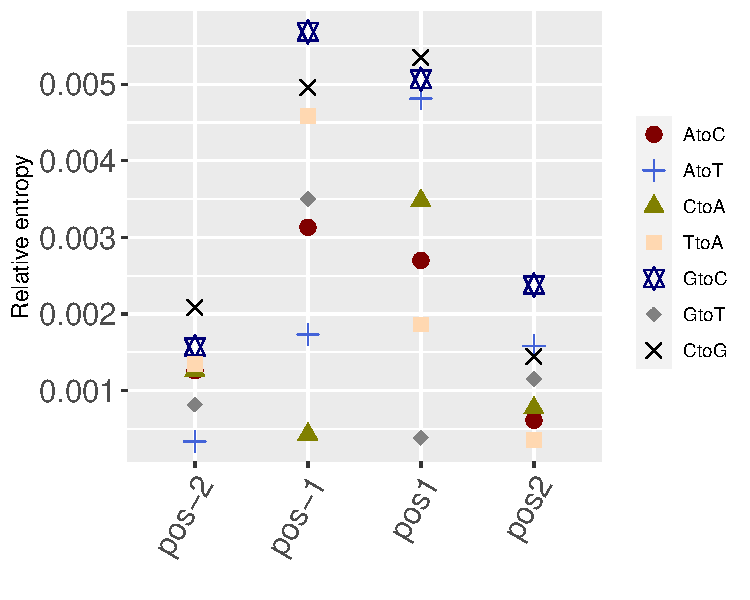
\includegraphics[scale=0.63]{graphics/nbr_transversion_Liver-HCC.pdf}
    \caption{transversion/Liver-HCC}
    \label{fig:transversion_liver}
    \end{subfigure} \\
    
    \caption{\textbf{Flanking bases were a good source of information.} Here, $RE$'s are shown for (a) transitions in Skin-Melanoma (b) transversions in Skin-Melanoma (c) transitions in Liver-HCC (d) transitions in Liver-HCC. The other cancers can be found in Figure \ref{fig:apdx_nbr}. For each panel, each dot was derived from a GLM. The x-axis is the flanking positions with respect to the substitution (substitution at 0); the y-axis is the $RE$ values.}
    \label{fig:nbr}
\end{figure}

\section{Chapter summary}